\documentclass{article}
\usepackage[T1]{fontenc}
\usepackage[utf8]{inputenc}
\usepackage[section]{placeins}
\usepackage{fullpage}
\usepackage{graphicx}
\usepackage{caption}
\usepackage{subcaption}

\graphicspath{ {./images/} }

\title{CS 4516 Group \#5: Bandwidth Trunking Using Layer 2 Devices\\Results}
\author{Jason Rosenman \and Louis Fogel \and Sam Abradi}
\date{}

\begin{document}
\maketitle
In order to measure the effectiveness of our approach, we will collect performance metrics on our switching approach.
We will compare the results of these metrics to the performance of an unmodified software switch.
Due to the fact that neither switch will be implemented in hardware, our results may be slightly different than a hardware implementation.
We are looking to compare the behavior of the network at saturation both with and without redundant links.
We are going to look at the goodput of these situations with and without congestion control.
\begin{figure}[ht]
	\centering
	\begin{subfigure}[b]{0.4\textwidth}
		\centering
		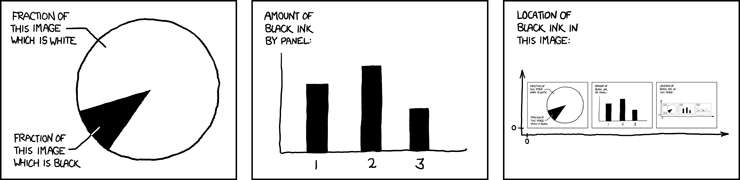
\includegraphics[scale=0.4]{self_description.png}
		\caption{Conventional Switch}
		\label{fig:stdbcast}
	\end{subfigure}
	\hfill
	\begin{subfigure}[b]{0.4\textwidth}
		\centering
		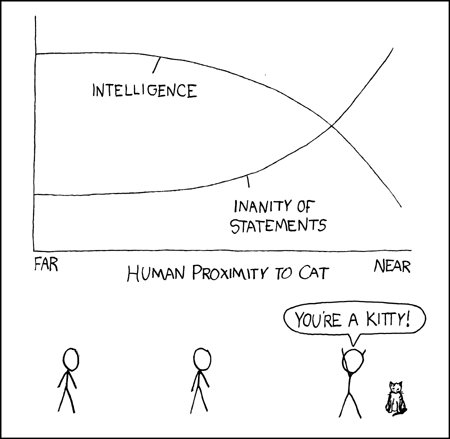
\includegraphics[scale=0.3]{cat_proximity.png}
		\caption{Smart Switch}
		\label{fig:newbcast}
	\end{subfigure}
	\caption{Percentage of Broadcast Traffic}
	\label{fig:bcast}
\end{figure}

\section{Congestion Conditions}
We expect that situations where the network is at saturation will show the biggest difference in performance between architectures. A setup with redundant links should perform much better than any other system if there is one flow causing all or most of the congestion, because all of the other traffic will default to the other link. Clearly single links are unable to provide this service, so they are going to have horrible performance in congestion conditions.
\section{Congestion Controll}
We have no idea what will happen in this situation.
\end{document}
